% polish: finishing touches: 
% 1. check spelling and grammar
% 2. Make line breaks look good
% 3. get figures where they need to be

% English Writing Center:
% - Start with main clause, when possible
% - Remove connectors: "Do I loose anything?". Don't use "so" - it's German!
% - Add commas after sentence connectors.
% - Don't use citations in sentences.
% - Try to keep out colloquial language ("Like this" -> "as follows")

\documentclass[a4paper,12pt]{article}

\usepackage[utf8]{inputenc}
\usepackage[ngerman, english]{babel}

\usepackage{mathtools, amssymb, amsthm, bbm}
\usepackage{hyperref}
\usepackage[
  labelfont=bf,
  labelsep=period,
  margin=10mm
]{caption}

\usepackage{graphicx}
\graphicspath{ {./assets/} }

\usepackage{biblatex}
\addbibresource{main.bib}

\usepackage{geometry}
\geometry{
  a4paper,
  top=2.5cm,
  bottom=2.5cm,
  left=2.5cm,
  right=2.5cm
}

\setlength{\parskip}{\medskipamount}
\setlength{\parindent}{0pt}
\setlength{\skip\footins}{6mm}
\sloppy

% Theorem definitions
\theoremstyle{plain}
\newtheorem{theorem}{Theorem}[section]
\newtheorem{lemma}[theorem]{Lemma}
\newtheorem{corollary}[theorem]{Corollary}
\newtheorem{proposition}[theorem]{Proposition}
\newtheorem{observation}[theorem]{Observation}
\newtheorem{conjecture}[theorem]{Conjecture}
\newtheorem{remark}[theorem]{Remark}

\theoremstyle{definition}
\newtheorem{definition}[theorem]{Definition}
\newtheorem{convention}[theorem]{Convention}
\newtheorem{example}[theorem]{Example}
\newtheorem{question}[theorem]{Question}
\newtheorem{problem}[theorem]{Problem}

% Symbol/Operator shortcuts
\def\R{\mathbb{R}}
\def\N{\mathbb{N}}
\def\B{\mathbb{B}}
\def\P{\mathcal{P}}
\def\xc{\operatorname{xc}}
\def\pc{\operatorname{pc}}
\def\dist{\operatorname{dist}}
\newcommand{\abs}[1]{\lvert#1\rvert}
\newcommand{\norm}[1]{\left\lVert#1\right\rVert}




\begin{document}

\pagestyle{empty}

\begin{titlepage}
\begin{center}

\includegraphics{TUMlschwarz.png}\\[3mm]
\sf
{\Large
  Technische Universit\"at M\"unchen\\[5mm]
  Department of Mathematics\\[8mm]
}
\normalsize
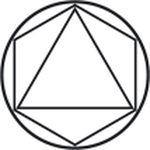
\includegraphics{TUMlMschwarz.png}\\[15mm]

Bachelor's Thesis\\[15mm]

{\Huge
  Extension Complexity of Convex n-gons
}
\bigskip

\normalsize

Josef Wittmann
\end{center}
\vspace*{75mm}

Supervisor: Prof. Dr. Stefan Weltge
\medskip

Advisor: Prof. Dr. Stefan Weltge
\medskip

Submission Date: \today
% todo: Insert actual date

\end{titlepage}

\vspace*{150mm}

I assure the single handed composition of this bachelor's thesis only supported by declared resources.
\bigskip

Munich, \today
\newpage

\section*{Zusammenfassung}
% todo @ March 21

Bei einer in englischer Sprache verfassten Arbeit muss eine Zusammenfassung in deutscher Sprache vorangestellt werden.
Daf\"ur ist hier Platz.

\newpage


\begin{otherlanguage}{ngerman}
  \section*{Zusammenfassung}
% todo @ March 21

Bei einer in englischer Sprache verfassten Arbeit muss eine Zusammenfassung in deutscher Sprache vorangestellt werden.
Daf\"ur ist hier Platz.

\newpage
\end{otherlanguage}

\tableofcontents
\newpage

\pagenumbering{arabic}
\pagestyle{plain}

\section*{Abstract}
In this paper we provide an overview of the current state of the extension complexity of convex $n$-gons (i.e., two-dimensional polytopes with $n$ vertices). First we give an overview of the lower bound ($xc(P_n) \geq \sqrt{n}$) and summarize the arguments, why this is true. Then we provide a geometric visualization of Shitov's proof that $xc(P_n) \leq \frac{6}{7}n$. From that we give a geometric proof of Shitov's result that $xc(P_n) \leq o(n)$ from which we improve the known upper bound for the extension complexity of $n$-gons slightly.


\section{Introduction} 

\subsection{Extension Complexity}

To describe a regular hexagon with linear inequalities, 6 of these are required. However by projecting a 3-dimensional polytope\footnote{A polytope is the convex hull of a finite set of points.}, one can describe the same polygon with 5 linear inequalities, see Figure~\ref{fig:hexagon}. 

\begin{figure}[h]
  \centering
  \includegraphics[scale=0.5,trim={0 2.5cm 0 2cm},clip]{assets/hexagon}
  \caption{A regular hexagon as a projection of a polytope with 5 factes (see \cite{kwan2020extension}).}
  \label{fig:hexagon}
\end{figure}

This is the key idea behind extended formulations. Simplifing the representation of polygons by projecting simpler (higher-dimensional) polytopes "down" to the desired polytope.
One can think of this operation as "compressing" the representation. This mental image is inspired by the fact, that regular $n$-gons (i.e. polygons with $n$ vertices), only require $O(\log(n))$ inequalities in their compressed form (see \cite{kaibel2010constructing}).

This intuition is formalized like this:

\begin{definition}[Extended Formulation]
  Let $P$ be a $d$-dimensional polytope, $Q$ a $m$-dimensional polytope and $\pi:\R^d \to \R^m$ a linear projection.
  The pair $(Q,\pi)$ is called an \textit{extended formulation} of $P$, if $\pi(Q)=P$. The \textit{size} of $(Q,\pi)$ is defined as the number of factes of $Q$.
\end{definition}

\begin{definition}[Extension Complexity]
  The \textit{extension complexity} of a polytope $P$ is the smallest possible size of an extended formulation of $P$. Is is usually denoted with $\xc(P)$.
\end{definition}

Polytopes with a small extension complexity can be "compressed" very well with extended formulations.
Such simplified formulations can be used for building faster algorithms for hard linear programs \cite{yannakakis1991expressing}.



\subsection{Overview of Current Research}

The application of extended formulations for solving hard linear problems seems promising. But reserach in the past years shows some unpromising examples:
\begin{itemize}
  \item It was shown in \cite{fiorini2015exponential}, that the \textit{traveling salesman} polytope can't have polynomial extension complexity. So here extended formulations don't provide an improvement over traditional methods.
  \item The results for the \textit{matching} polytope are even worse: In contrast to the polynomial-time algorithm (\cite{ford1956maximal}) for solving this problem, there is no polynomial-size extended formulation (\cite{rothvoss2017matching}).
\end{itemize}

So the study of polyons has importance as a benchmark for extened formulations in general (Braun and Pokutta called this "prototypical importance" in \cite{braun2015matching}).
That's why current research focuses on finding good bounds for the extension complexity, rather than developing algorithms for constructing such extensions.

There are currently two main approaches for finding bounds for the extension complexity: The first one is the natural geometric approach. The second one is a linear algebraic approach based on a remarkable result of Yannakakis in \cite{yannakakis1991expressing}, which we'll recall briefly:

\begin{definition}[Slack Matrix]
  Let $P$ be a polytope.
  Then a \textit{slack matrix}\footnote{Note that the slack matrix depends on the representation of $P$. So there is no single slack matrix to a given polytope.} $M$ of $P$ is a nonnegative matrix whose rows are indexed by the vertices of $P$ and whose columns are indexed by the linear constraints of some representation of $P=\{x \in \R^d \mid Ax \leq b\}$. 
  The entries of $M$ are defined as $m_{ij} = b_j - a_j v_i$, where $a_j$ is a row of $A$ and $v_i$ is a vertex of $P$.
\end{definition}

\begin{definition}[Nonnegative Rank]
  The \textit{nonnegative rank} of a nonnegative matrix $M \in \R^n \times \R^m$ is the smallest integer $k$, for which $M = TU$, where $T \in \R^n \times \R^k$ and $U \in \R^k \times \R^m$.
  We define $rank_+(M) := k$.
\end{definition}

\begin{theorem}[see \cite{yannakakis1991expressing}]
  Let $P$ be a polytope and $M$ a slack matrix of $P$. Then $\xc(P) = rank_+(M)$.
\end{theorem}

Because this document is focused on polygons, we briefly recall the history of bounds and conjectures for the extension complexity of $n$-gons:

Define $\P_n$ as the set of all convex polygons with $n$ vertices. Then $$\pc:\N \to \N, \pc(n) = \max \{\xc(P) \mid P \in \P_n\}$$ is called the \textit{polygon complexity}, i.e. the largest extension complexity for a polygon of size~$n$.

The lower bound $\pc(n) \in \Omega(n^{1/2})$ is quite easy to prove, which was done by the authors of \cite{fiorini2012extended} by a counting argument. In this paper we will provide another approach to proving this lower bound. 

But the upper bound is more challenging. Only few improvements have been made for a long time and the trivial upper bound $\pc(n) \leq n$ could only be improved by constant factors. One such improvement was done independently by Shitov \cite{shitov2014upper} and Padrol \& Pfeifle \cite{padrol2014polygons} and proved that $\pc(n) \leq (6n+6)/7$. The basis for their prove was the fact that $\pc(7)=6$, i.e. each heptagon has extension complexity at most 6.

Because of missing improvements it was conjectured, that $\pc(n) \in \Theta(n)$ (see \cite{fiorini2012extended}). This was falsified by Shitov by proving $\pc(n) \in o(n)$ in \cite{shitov2014sublinear}. He later improved the upper bound to $\pc(n) \in O(n^{2/3})$ in \cite{shitov2020sublinear}, which is the best known bound so far.

In summary, this is currently known about the polygon complexity:
$$\pc(n) \in \Omega(n^{1/2}) \cup O(n^{2/3})$$

There is another recent paper \cite{kwan2020extension}, which focuses on cyclic polygons\footnote{A polygon is called cyclic, if all its vertices lie on a circle.}. The authors proved that $\xc(P) \in O(n^{1/2})$ for all cyclic $n$-gons. 
This led the authors to propose, that this upper bound could also hold for general $n$-gons, since "cyclic polygons seem to represent quite a diverse cross-section of the space of all polygons".



\subsection{Overview of this Document}

% cite papers
In this paper we focus on the key ideas behind the discussed papers \cite{shitov2020sublinear,kwan2020extension}. We will make use of examples and skip technical details.

In the first part we examine the results that led to the best known upper bounds. 
We will start with Shitov's paper \cite{shitov2020sublinear}, which provides the upper bound of $O(n^{2/3})$ with a purely geometric approach.
From there we have a look at cyclic n-gons and the upper bound of $O(n^{1/2})$, which was provided by a semi-geometric / semi-algebraic approach in \cite{kwan2020extension}.
Next we try to compare these two approaches, as far as they are comparable. First on a high level -- comparing key ideas -- and later on a more technical level.

In the second part we give another proof of the lower bound and present the utilized theorem \cite[Theorem 1]{averkov2016maximum}, which can be applied on various problems. We also give a quick overview of the key ideas behind this theorem.


\section{Upper Bounds for the Extension Complexity}
% todo @ March 12 to 18
% todo: skip overview, since it is provided at the end of introduction
% todo: choose right fraction (\frac or "/") to look nice (ctrl+F)
% todo: add citations from original paper (to every definition, theorem, ...)
% todo: maybe add sum subsubsections?

\subsection{Arbitrary Convex n-gons}
% todo @ March 13 to 15

In this section we give a detailed overview of \cite{shitov2020sublinear}, which proofs $\pc(n) \in O(n^{2/3})$ for arbitrary $n$-gons. 
We focus on the underlying ideas and present only important arguments in more detail. In contrast to the source, we present the proof "backwards", starting from the results, since in doing so we can highlight the reasoning more clearly.

% todo: Maybe give overview (split, subsequence, glueing simple extension)

The starting point is the following lemma, adpopted from \cite[Proposition 3.1.1]{weltge2015sizes}, which states that $\xc$ behaves well for unions of polytopes:
\begin{lemma}\label{lemma:union}
  Let $P$ and $Q$ be polytopes in $\R^d$ -- each different from a point \footnote{In regards to polygons, one is tempted to think of these polytopes as being disjunct. But they can be arranged arbitrarily}. Then $$\xc(\conv(P \cup Q)) \leq \xc(P) + \xc(Q) .$$
\end{lemma}

This allows us to split the polygon into smaller pieces with small extension complexity. Joining them together will transfer this good extension complexity to the original polygon.

Now we will go on to define those smaller pieces, which we can handle well.

\begin{definition}[Thin sequence]
  % todo: Formulate + examples
\end{definition}
\begin{observation}[Splitting into thin sequences]\label{observation:splitting}
  % todo: formulate + image
\end{observation}

Based on Observation~\ref{observation:splitting} we choose to split the $n$-gon into $12$ distinct $pi/6$-thin sequences. Joining those (constantly many) sequences will not change the extension complexity of the original polygon in light of Lemma~\ref{lemma:union}. \\
Now we will go on to show that each sequence has extension complexity $O(n^{2/3})$.

\begin{theorem}\label{theorem:subsequence}
  Let $v$ be a $\pi/6$-thin sequence with $n = 1024\tau^3 + 8\tau$ vertices, where $\tau \in \N$. 
  Then $v$ contains a subsequence $u$ with $\abs{u} \geq 4\tau^2$ and $\xc(u) \leq 12\tau$.
\end{theorem}
% todo: explain that proof comes later

% todo: explain motivation/idea
\begin{corollary}\label{corollary:subsequence}
  Let $v$ be a $\pi/6$-thin sequence with $n > 263 000$ vertices. 
  Then $v$ contains a subsequence $u$ with $\abs{u} \geq \frac{1}{36} n^{\frac{2}{3}}$ and $\xc(s) \leq \left( \frac{72}{43}n \right)^{\frac{1}{3}}$.
\end{corollary}
% todo: proof (sketch)

% todo: explain idea (induction)
\begin{corollary}\label{corollary:thin-xc}
  Let $v$ be a $\pi/6$-thin sequence. Then $\xc(v) \leq \frac{324}{\sqrt[3]{129}} n^{\frac{2}{3}}$.
\end{corollary}
% todo: proof (sketch)

% todo: summarize idea
\begin{theorem}\label{theorem:xc}
  Every convex $n$-gon $P$ has $\xc(P) \leq 147 n^{\frac{2}{3}}$.
\end{theorem}
% todo: proof


Before we can determine the subsequences in Theorem~\ref{theorem:subsequence}, we need to find a way to build those extended formulations.

The key idea here is to omit some vertices to obtain a simpler surrounding polygon. For this polygon we build extended formulations with respect to the omitted vertices. If we now "glue" those extended formulations together in a special way, we get an extended formulation for the original polygon with small extension complexity.

Before we can formulate this theorem, we have to introduce \emph{acute polyhedra} and acute diagrams. These help us build the extensions for the (simple) surrounding polygon.
% todo: Explain acute diagrams and the idea behind them.
% todo: State/explain Lemma 26

% todo: introduce Theorem 28 (idea, application and reference to image)
\begin{theorem}[Glueing acute extensions together, {\cite[Theorem 28]{shitov2020sublinear}}]
  Let $P$ be a polygon with vertex set $V$ and $\emptyset \neq S \subset V$ be a proper subset of all vertices. Fix $\delta \geq 1$. Assume that

  (i) for any $s \in S$ there are two vertices $s'$, $s''$ on two edges of $P$ adjacent to $s$.

  (ii) there are $\delta$ points $\left\{s^1, \dots, s^\delta \right\}$ in the interior of the triangle ${T_s = \conv \left\{s,s',s''\right\}}$.
  
  (iii) the triangles $T_s$ are disjoint for different $s$.

  (iv) for any $i \in \{1,\dots,\delta\}$ there exists and acute diagram $D^i$ with base face $P$ such that, for any $s \in S$, the segment between $s$ and $s^i$ is a subset of the main edge of $D^i$ passing from $s$. 
  
  Then $$\xc\left( \conv\left( (V \setminus S) \cup \bigcup_{s \in S} \left\{ s',s'',s^1,\dots,s^\delta \right\}  \right) \right) \leq \abs{V} + \abs{S} + \delta .$$
\end{theorem}
% todo: image of theorem 28
% todo: proof theorem 28

% todo: Limits of Theorem 28: $O(n^{1/2})$
% todo: Note the difference in Theorem 28 ("contains") and Lemma 26 ("direction") and note that it's not compatible
% todo: explain G-good and Lemma 42 (ray definition of "good")

% todo: Return to sequences
% todo: We look at two cases: Slanted and unslanted sequences
% todo: State that both have (big enough) subsequences which can utilize Theorem 28 well (the asymptotical optimum for Theorem 28 is achived) --> Glimpse of chapters 9 to 11

% todo: summarize 
% todo: possible improvements, applications

\begin{itemize}
  \item What is the key idea?
  \begin{itemize}
    \item splitting n-gons into (constantly many) thin slices
    \item Inductively extracting subsets (vertices not neccessarily in order) with small extension, since $\xc(\conv(P \cup Q)) \leq \xc(P) + \xc(Q)$, repeatedly
    \item Bounding $\xc$ of those subsets (either it's "slanted" or not)
    \item Constructing and glueing 3-d extended formulations: Theorem 28
    \item Considering simple extensions ("liftings") by looking at acute diagrams
    \item Finding subsets, which are "good" in regards to Theorem 28
  \end{itemize}
  \item Essential statements
  \begin{itemize}
    \item Existence of an acute diagram with all but one direction fixed (Lemma 26)
    \item Theorem 28
    \begin{itemize}
      \item What does it say?
      \item Maximum possible result with Theorem 28: $O(n^{1/2})$ (it is achived for the extracted subsequences)
      \item Why can't one just apply Theorem 28 (and skip the rest of the paper)? Cue: "contains"
    \end{itemize}
    \item Requirements of Theorem 28
    \begin{itemize}
      \item G-good = Theorem 28 applicable (acute diagram exists)
      \item Rays leave through upper edge = acute diagram exists (Lemma 42)
    \end{itemize}
    \item Good upper bounds for slanted/not slanted subsequences
  \end{itemize}
  \item Proofs worth repeating
  \begin{itemize}
    \item I guess Theorem 28 :)
    \item Lemma 42 (good = ray)?
    \item Lemma 48?
    \item Lemma 25 / Corollary 26?
  \end{itemize}
  \item Examples worth making/drawing
  \begin{itemize}
    \item all examples from source
    \item Examples of acute polytope/diagram (main edges + orientation in most proofs)
    \item Examples of thin sequences (one thin, one not thin and one thin with one side > 90 deg)
    \item Ray $\rho$
    \item G-envelope + G-good
    \item Slanted sequences: angle $\beta$
    \item Decreasing sequence?
    \item Perfect sequence
  \end{itemize}
\end{itemize}

\begin{tabular}{| p{50mm} | p{100mm} |}
  \hline
  \multicolumn{2}{|c|}{\textbf{Main results per chapter}}\\ \hline
  3. Preliminaries & Extension Complexity for union of polytopes \\ \hline
  4. Acute polyhedra & There is an acute polyhedron for a polygon, where all main edges except one have fixed direction \\ \hline
  5. Acute diagrams & There is an acute diagram for a polygon, where all main edges except one have fixed direction \\ \hline
  6. Glueing acute extensions together & Skip vertices of a polygon by joining acute diagrams to get an extended formulation which represents the original polygon \\ \hline
  7. Thin sequences & Splitting polygons is now a thing \& something about rays passing a horizontal line \\ \hline
  8. Good sequences & good sequences let you apply Theorem 28, identify good sequence via ray passing through top \\ \hline
  9. Extracting a slanted subsequence & When it's not slanted, it'll extend well (Lemma 49) \\ \hline
  10. Decreasing slanted sequences & Get estimates of xc for slanted sequences \\ \hline
  11. Extensions for slanted sequences & Subsequence of slanted sequence with good xc \\ \hline
  12. Completing the proof & Split the polygon, iteratively extract a subsequence and bound xc (see chapter 11 for slanted, chapter 9 for not slanted) \\ \hline
\end{tabular}



\subsection{Cyclic n-gons}
% todo @ March 16 to 18

\begin{itemize}
  \item overview of paper
  \item What is the key idea?
  \item coloring
  \item intuition of rescaling rows
  \item Higher-dimensional statements
\end{itemize}



\subsection{Comparison}
% todo @ March 19 to 20

\begin{itemize}
  \item general similarities (splitting of polygons, bulging of corners)
  \item general differences (splitting by angle vs count, coloring and independece of slices in general case)
  \item How is the circle property used? Can the approach be generalised?
  \item could the general case be $O(\sqrt{n})$, too? (current conjectures)
  \item Is there a way to adopt a proof to the other case? Try Shitov's work on cyclic polygons.
\end{itemize}


\section{Lower Bounds for the Extension Complexity}
% todo: Think about multi-dimensional proof

In this section we provide yet another proof for $pc(n) \in \Omega(n^{1/2})$.

After the proof is done, we will explain the key concepts of the applied theorem and show how to apply it in general.

The central piece of the proof is Theorem~1 from \cite{averkov2016maximum}, which we adopt for the case of linear extended formulations (the original also allowed semidefinite ones).

Therefore we have to introduce the \textit{Hausdorff distance} of two non-empty compact sets $X,Y \subseteq \R^d$, which can be thought of "the longest distance you can be forced to travel from a point in one of the two sets to the other set". See Figure~\ref{fig:hausdorff} for an example.

\begin{figure}[h]
  \centering
  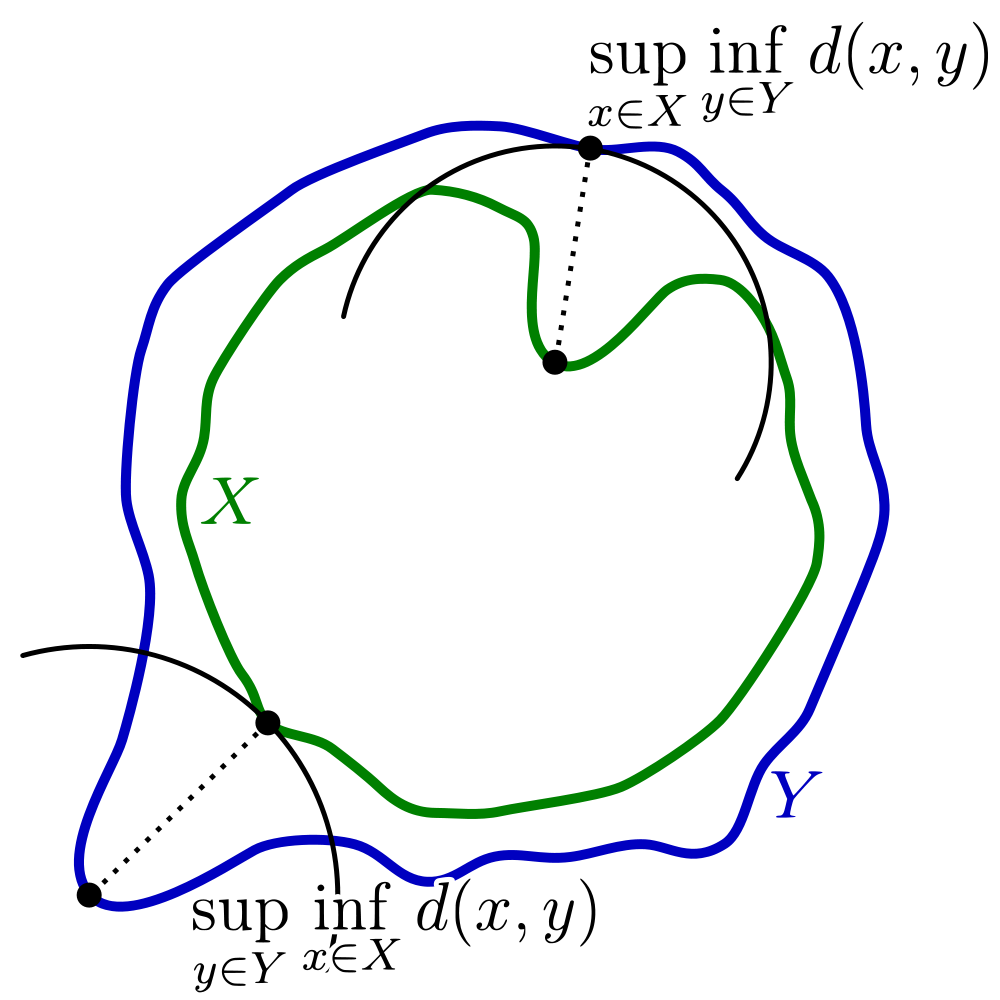
\includegraphics[height=55mm]{assets/Hausdorff_distance.png}
  \caption{Hausdorff distance example \cite{rocchini2007hausdorff}}
  \label{fig:hausdorff}
\end{figure}

\begin{definition}[Hausdorff distance]
  The \textit{Hausdorff distance} with respect to the Euclidean norm is defined by $$ \dist_H(X,Y) := \max \left\{ \sup_{x \in X} \inf_{y \in Y} \norm{x-y}, \sup_{y \in Y} \inf_{x \in X} \norm{x-y} \right\} .$$
\end{definition}

\begin{theorem}[{\cite[Theorem 1]{averkov2016maximum}}, adopted]\label{theorem:family}
  Let $\P$ be a family of polytopes in $\R^d$ of dimensions at least one with $2 \leq \abs{\P} < \infty $ such that each $P \in \P$ has an extended formulation of size $m$.
  Let $\rho > 0$ and $\Delta > 0$ be such that each $P \in \P$ is contained in the ball $\rho \B^d$ and, 
  for every two distinct polytopes $P \in \P$ and $P' \in \P$, one has $\dist_H(P, P') \geq \Delta$. 
  Then $$m^2 \geq \frac{\log_2 \abs{\P}}{8d \left(1 + \log_2 (2\rho/\Delta) + \log_2\log_2 \abs{\P} \right)} =: B.$$
  In particular, we have $$\max \{\xc(P) \mid P \in \P\}  \geq \sqrt{B} .$$
\end{theorem}



\subsection{Proof of Lower Bound}

\begin{corollary}
  $pc(n) \in \Omega(\sqrt{n})$
\end{corollary}
\begin{proof}
  To apply \ref{theorem:family} we have to pick a familiy of polytopes $\P$. Then we have to determine $\rho$ and $\Delta$ and bound $\log_2 \abs{\P}$ from below and $\log_2 \log_2 \abs{\P}$ from above.

  So we choose $n^2$ fixed points evenly on the unit circle (so they would form a regular polygon). Let $\P_n$ be the familiy of polygons, where each polygon has $n$ vertices chosen from the $n^2$ points on the unit circle.

  Then $\rho = 1$, since all polygons are contained in the unit circle.

  For two distinct polygons $P, P' \in \P_n$ one of them has a vertex $v$, which the other one does not have. W.l.o.g $v \notin P, v \in P'$. So $\dist_H(P,P') \geq \inf_{p \in P} \norm{v-p} \geq d_{min}$ (see Figure~\ref{fig:distance} for the definition of $d_{min}$).

  \begin{figure}[h]
    \centering
    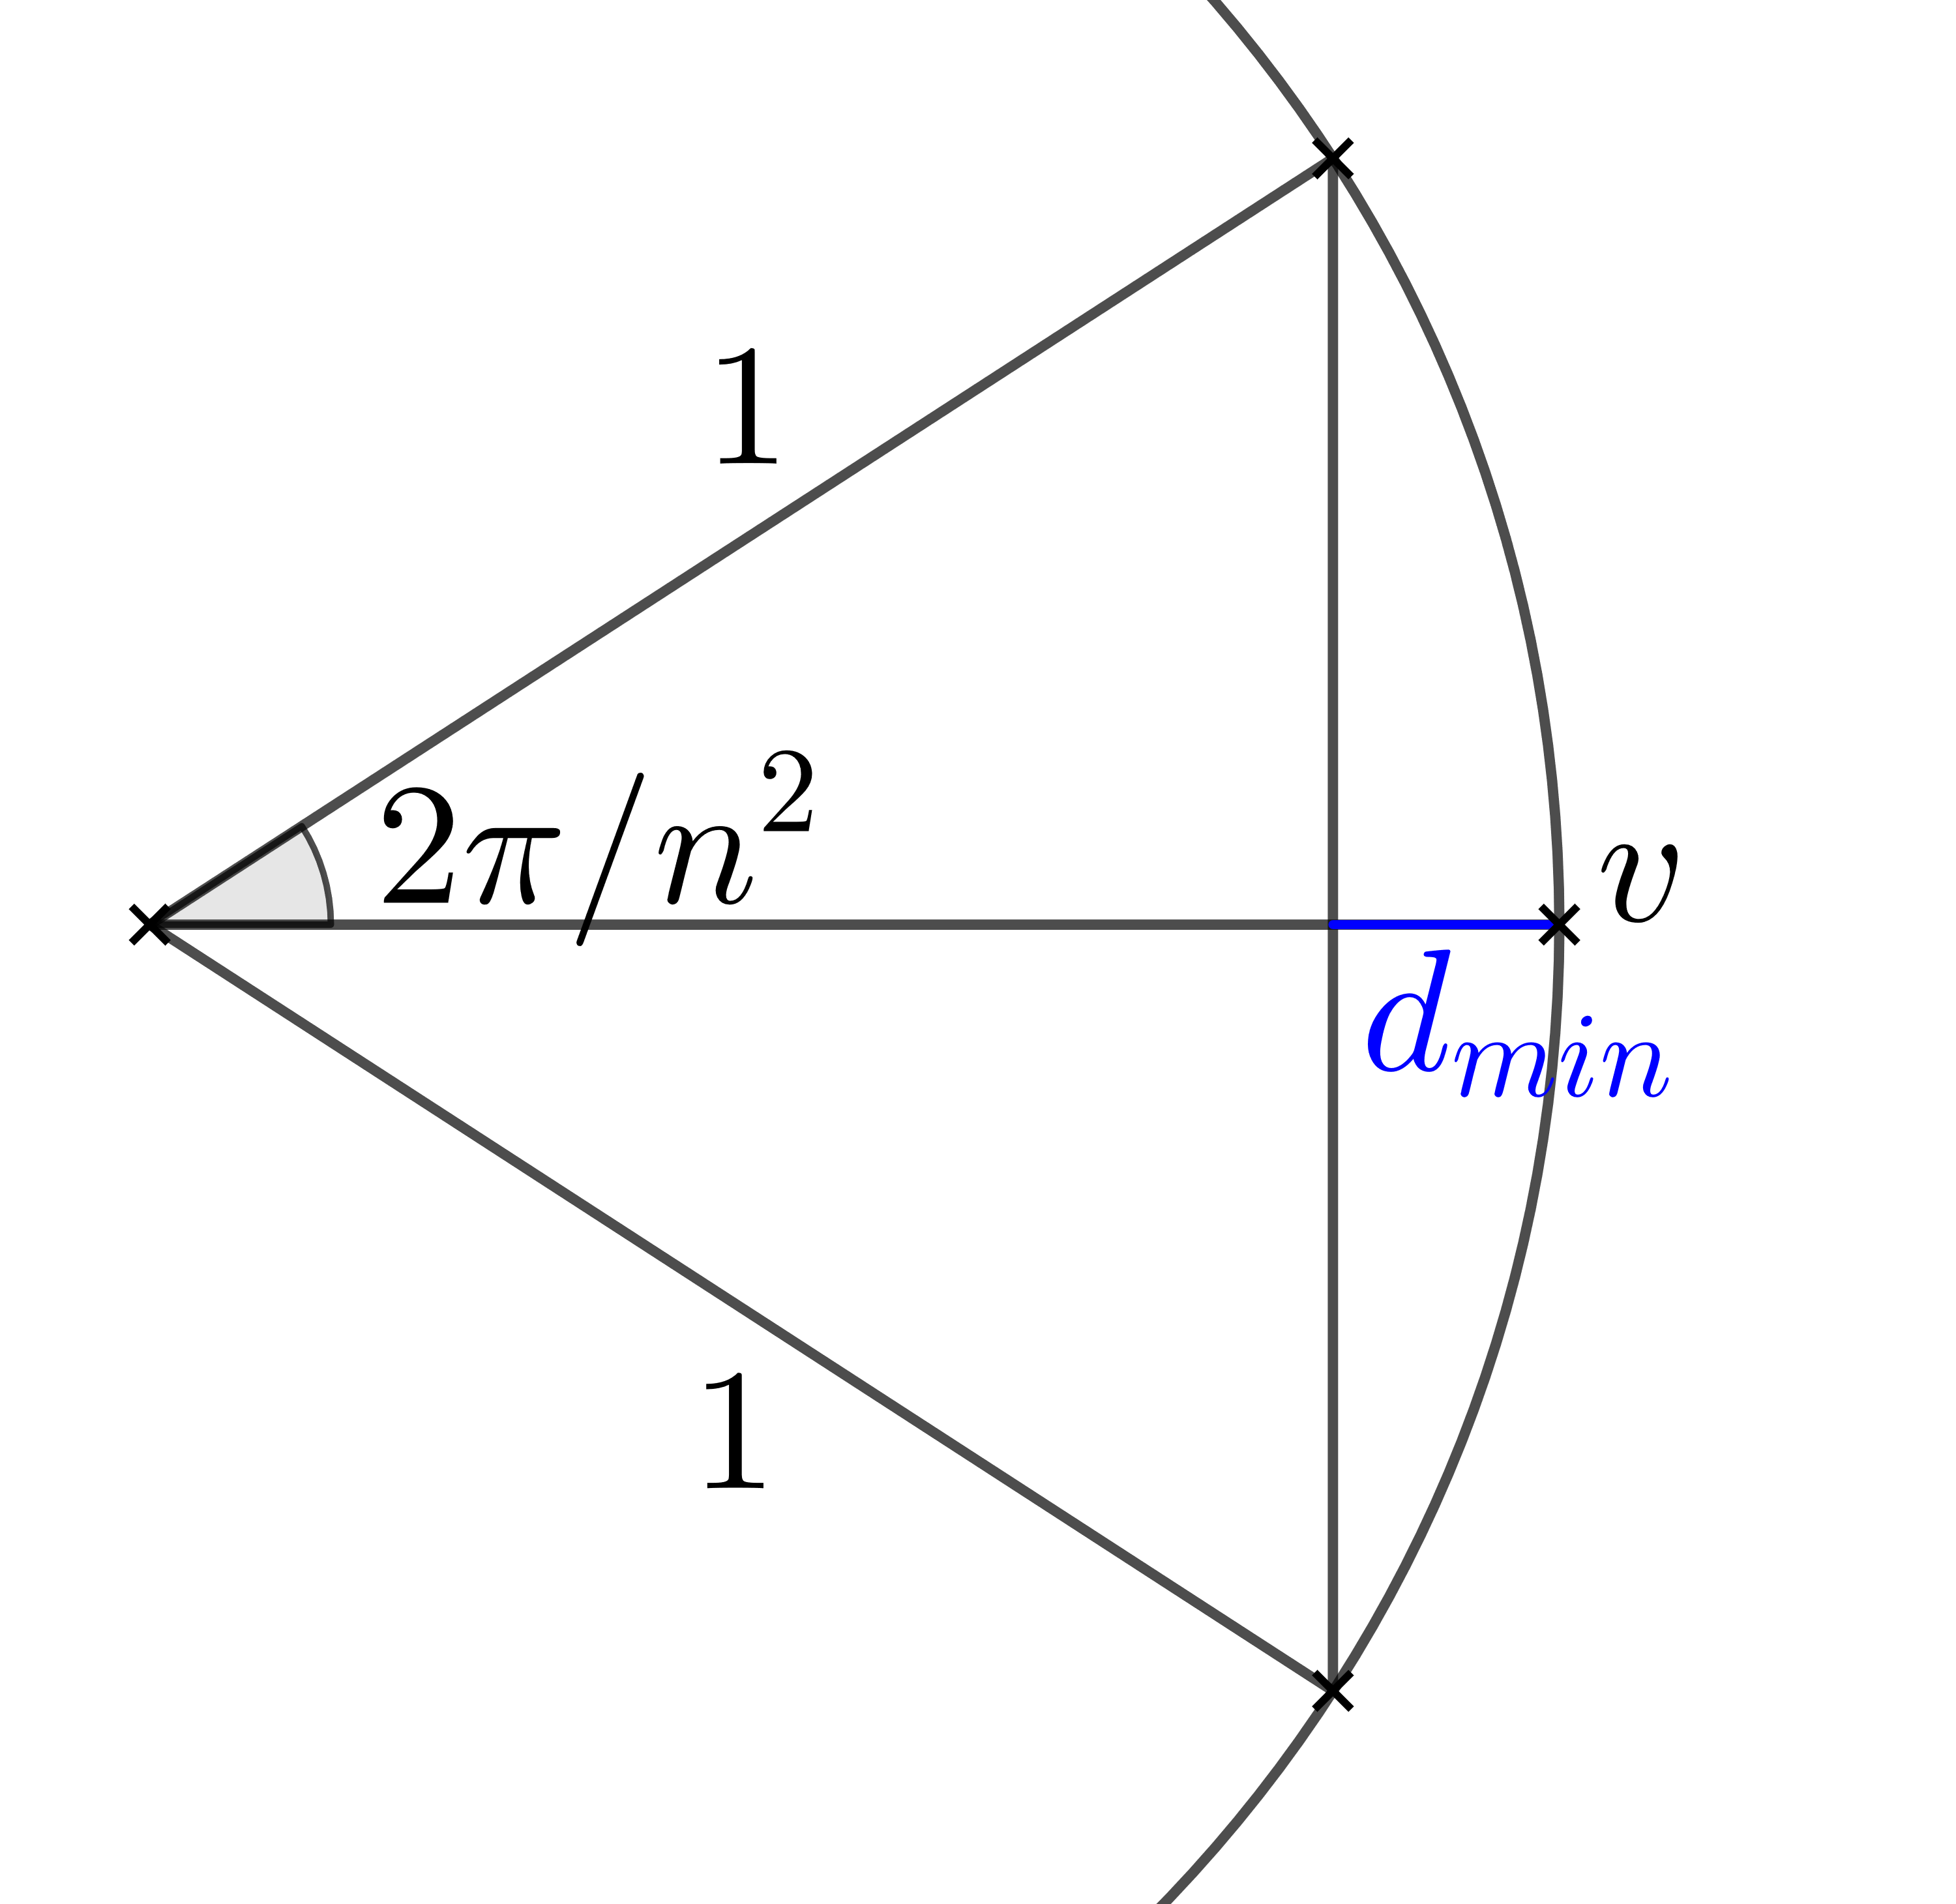
\includegraphics[height=55mm]{assets/Minimal_Hausdorff_distance.png}
    \caption{Definition of $d_{min}$}
    \label{fig:distance}
  \end{figure}
  
  \begin{align*}
    1 - d_{min} &= \cos\left( \frac{2 \pi}{n^2} \right)\\
    d_{min} &\geq 1 - \left(1 - \frac{\left(\frac{2 \pi}{n^2}\right)^2}{2} \right) = 2 \frac{\pi^2}{n^4} =: \Delta
  \end{align*}

  For the estimate we used $\cos(x) \leq 1 - \frac{x^2}{2!}$, which arises from the power series for cosine.

  Since each polygon in $\P_n$ is defined by $n$ points, chosen from a set of $n^2$ points, $\abs{\P_n} = \binom{n^2}{n}$. Therefore $n^n = \left( \frac{n^2}{n} \right)^n \leq \abs{\P_n} \leq \left( n^2 \right)^n = n^{2n}$. $\log_2 \abs{\P_n} \geq n \log_2 n$ and $\log_2 \log_2 \abs{\P_n} \leq \log_2 (2n \log_2 n) = 1 + \log_2 n + \log_2 \log_2 n$.

  Now we can calculate $B$ from Theorem~\ref{theorem:family}:
  \begin{align*}
    B &= \frac{\log_2 \abs{\P_n}}{8d \left(1 + \log_2 (2\rho/\Delta) + \log_2\log_2 \abs{\P_n} \right)}\\
    &\geq \frac{n \log_2 n}{16 \left(1 + \log_2 (n^4 / \pi^2) + 1 + \log_2 n + \log_2 \log_2 n \right)}\\
    &= \frac{n \log_2 n}{16 \left(2 - 2 \log_2 \pi + 5 \log_2 n + \log_2 \log_2 n \right)}\\
    &\geq \frac{n}{16*6}
  \end{align*}

  For the last inequality we used $2 - 2 \log_2 \pi \leq 0$ and $\frac{5 \log_2 n + \log_2 \log_2 n}{\log_2 n} \leq 6$ for $n \geq 1$.

  Therefore we can conclude $$\pc(n) \geq \max \{\xc(P) \mid P \in \P_n\} \stackrel{\text{(Th. \ref{theorem:family})}}{\geq} \sqrt{B} \geq \frac{1}{12} \sqrt{n} .$$
\end{proof}



\subsection{Key Ideas Behind the Applied Theorem}
% todo: formulate

\begin{enumerate}
  \item Encode polytopes trough normalized extended formulations (Everything from now on in encoding vector space)
  \item Bound pairwise distance from below (using $\Delta$)
  \item Draw spheres around enconding point (half of min distance)
  \item Bound radius of containing ball from above (using $\rho$)
  \item Bound maximum number of possible by volume (how many encodings can fit in containing ball)
\end{enumerate}


\section{Concluding Remarks}

In this paper we looked at the best known bounds for the extension complexity of polygons.

For cyclic polygons $P$ we know $\xc(P) \in \Theta(n^{1/2})$.

For arbitrary polygons $P$, we only know $\xc(P) \in \Omega(n^{1/2}) \cap O(n^{2/3})$.

\textcite{kwan2020extension} conjectured that cyclic polygons have worst-case extension complexity, i.e.\ $\xc(P) \in \Theta(n^{1/2})$, because they ``seem to represent quite a diverse cross-section of the space of all polygons'' \cite[3]{kwan2020extension}.

On the other hand, \textcite{shitov2020sublinear} expected that $\pc(n) = n^{1/2} \cdot \alpha(n)$ with unbounded $\alpha(n)$ \cite[Conjecture 61]{shitov2020sublinear}.

He reasons that the method developed in his paper doesn't seem to allow an $O(n^{1/2})$ upper bound for the worst-case $n$-gon complexity. This means there is no subsequence of $\Theta(n)$ vertices, for which we could apply Theorem~\ref{theorem:gluing} optimally.

And he also goes on explaining that \textcite{padrol2016extension} proved
\begin{equation}\label{eq:wcc}
  \wcc(d,n) \geq 2\sqrt{dn-d}-d+1 ,
\end{equation}
where $\wcc(d,n)$ is the largest possible extension complexity of a polytope with $n$ vertices in a $d$-dimensional space.
If the conjecture were false, the bound in \eqref{eq:wcc} would become asymptotically optimal for $d=2$, which is not expected, since \textcite{kaibel2015short} showed $\wcc(m^2,2^m) \geq 1.5^m$ for the \emph{correlation polytope} (This is asymptotically much greater than $(\sqrt{2})^m$, which is the result of equation \eqref{eq:wcc} in that case).

Thus, the question of worst-case extension complexity of polygons remains exciting.


\appendix
\section{Proof Dependency Graph}\label{sec:dependency-graph}

The following graph gives an overview of the dependencies in the proofs of \cite{shitov2020sublinear}.

Each node corresponds to a theorem, lemma or corollary given by its number.
Each edge indicates a dependency on the statement it is directed at. 
And the boxes group statements from different sections (``Sec.'' is short for ``Section'').

Definitions are omitted, as they would make the graph too crowded. 
Also, some edges could be missing, because dependencies aren't always obvious, when one is immersed in a subject for some time.

\includegraphics{dependency-graph}

\newpage

\printbibliography

\end{document}
